%%%%%%%%%%%%%%%%%%%%%%%%%%%%%%%%%%%%%%%%%%%%%%%%%%%%%%%%%%%%%%%%%%%%%%%%%%%%%
\section{Introduction}
\label{sec:intro}
Provided is a documentation of a new and recently developed Oslofjord model called FjordOs CL. FjordOs CL is based on version 3.6 of the Regional Ocean Modeling System - ROMS \citep{haidv:etal:2008, shche:mcwil:2005, shche:mcwil:2009} utilizing its curvilinear option. The model is developed as part of the project "New Oslofjord model for prediction of currents, water level and hydrography, here applied on oil spill preparedness and harbor development - FjordOs"\footnote{\texttt{http://www.fjordos.no}}. FjordOs is a cooperation between MET Norway, University College of  South-East Norway (HSN), NIVA, Kystverket, Exxonmobil, Norwegian Defence Research Establishment (FFI), Vestfold, Buskerud, and {\O}stfold county and AGNES AB Miljøkonsulent.. 

\subsection{The Oslofjord}
\label{subsec:oslofjord}
The Oslofjord is located in Southern Norway and is about 100 km long (Figure \ref{fig:map_oslofj}). Its width varies from about 25 km at the entrance ($\sim$ 59$^\text{o}$N) to about 1-2 km in the {\DR} Sound and {\DR} area. The fjord's main sill, which is marked by the horizontal bar in Figure \ref{fig:map_oslofj} (hereafter the {\DR} Sill), is located two thirds inside of the entrance to the fjord. This makes the Oslofjord peculiar among Norwegian fjords in that most of them have the sill at the entrance to the fjord. 
% %%%%%%%%%%%%%%%%%%%%%%%%%% Figure Map_location_Oslofjord %%%%%%%%%%%%%%%%%%%%%%%%%%%%
\begin{figure}[h]
 \setlength{\unitlength}{1.0cm}
 \begin{center}
  \begin{pspicture}(0,0)(15,9)
% Include graphs
   \rput[bl](-0.1,1.0){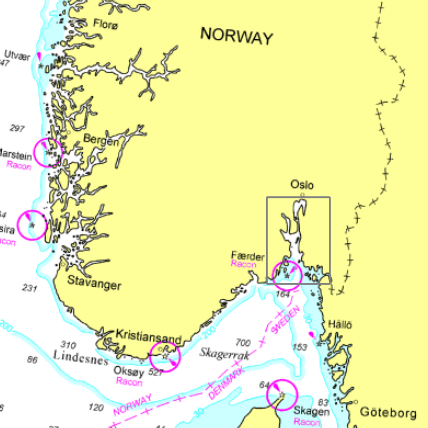
\includegraphics[height=7.3cm]{Map_location_Oslofjord_2}}
   \rput[br](15.0,0.0){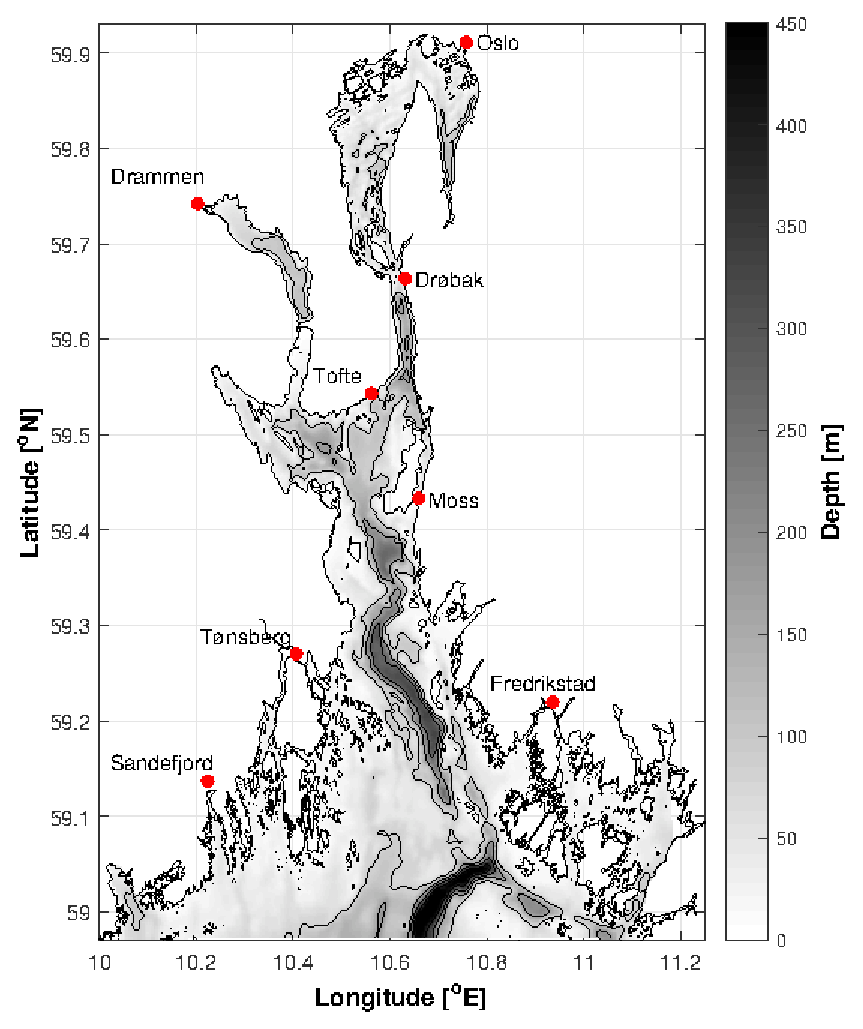
\includegraphics[height=9cm]{dyp_old}}
   \psline[linewidth=0.5mm,linecolor=blue]{->}(13.4,5.3)(11.3,6.3)
   \psline[linewidth=0.2mm](4.45,4.95)(7.5,8.5)
   \psline[linewidth=0.2mm](4.45,3.5)(7.5,1)
  \end{pspicture}
% Figure caption is below the figure
  \caption{\small The topography and irregular coastline of the Oslofjord and its location in Southern Norway. The right-hand gray scale bar indicates depth in meters. The blue arrow points to the location of the fjord's main sill (the {\DR} sill as enlarged in Figure \ref{fig:droebak_sill}) which is only $\sim$ 20 m deep. Note also the $\sim$ 400 m deep basin extending from the Skagerrak towards the Hvaler Archipelago in the southeast, the so called Hvalerdjupet. }
  \label{fig:map_oslofj}       % Give a unique label
 \end{center}
\end{figure}
%


The {\DR} Sill is partly man made\footnote{The jetty was built in the years 1874 - 1879 as a naval defense of Oslo, the capital of Norway. It forces large vessels to sail east of the fortress Oscarsborg built at Kaholmen.} and partly natural. The natural sill is about 20 m deep, while the man made part is only 1-2 m deep. The latter consists of an underwater barrier, the {\DR} Jetty, extending halfway across the {\DR} Sound from the western mainland south of {\DR} to south of the small island Kaholmen located slightly to the east of the southern tip of the {\HAA} (Figure \ref{fig:droebak_sill}). There are two narrow openings in the Jetty with a maximum depth of about 6 m. One is located close to the mainland on the western side, while the second runs east-west and is located just south of Kaholmen.   
%%%%%%%%%%%%%%%%%%% Figure 2 Bathymetry and currents in the Drøbak area %%%%%%%%%%%%%%%
\begin{figure}[t]
 \begin{center}
  \begin{pspicture}(0,0)(15,9)
% Include graphs
   \rput[b](7.5,0){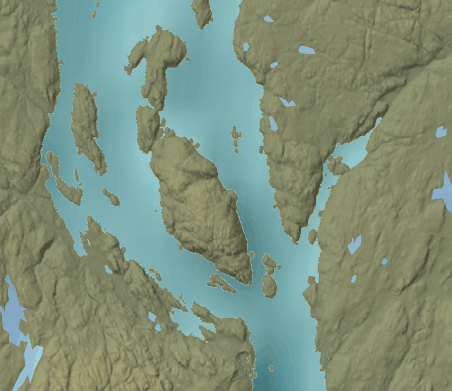
\includegraphics[height=9cm]{dyp_Drobak}}
   \rput[b](11,0){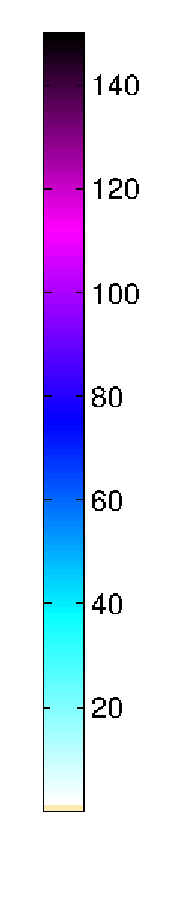
\includegraphics[height=9cm]{Fig02_color_bar}}
  \end{pspicture}
  \caption{\small The irregular coastline and topography in the {\DR} Sill area. The color bar indicates depth in meters.}
  \label{fig:droebak_sill}
 \end{center}
\end{figure}

 

The sill area represent a major obstruction for the water exchange between the inner and the outer part of the fjord. Due its narrowness and shallowness the {\DR} Sill area is famous for its strong tidal currents that easily exceeds 1 m/s. We also note that north of the sill the fjord is separated by {\HAA} into an eastern and a western channel each about 1 km wide. These channels and the openings in the Jetty are important to include in any model of the Oslofjord to obtain realistic circulation patterns and strengths in the area. Another noteworthy topographic feature is the Hvalerdjup located at the entrance to the fjord (Figures \ref{fig:map_oslofj} and \ref{fig:ferder_hvaler}). It is a 400 m deep basin extending northeastward from the Skagerrak towards the Hvaler Archipelago. As revealed by Figure \ref{fig:map_oslofj} there are also several other somewhat shallower basins $\sim$ 150 - 200 m deep as we proceed into the fjord. 
%%%%%%%%%%%%%%%%%%% Figure 2 Bathymetry and currents in the Drøbak area %%%%%%%%%%%%%%%
\begin{figure}[t]
 \begin{center}
  \begin{pspicture}(0,0)(15,8.5)
% Include graphs
   \rput[bl](-0.1,0){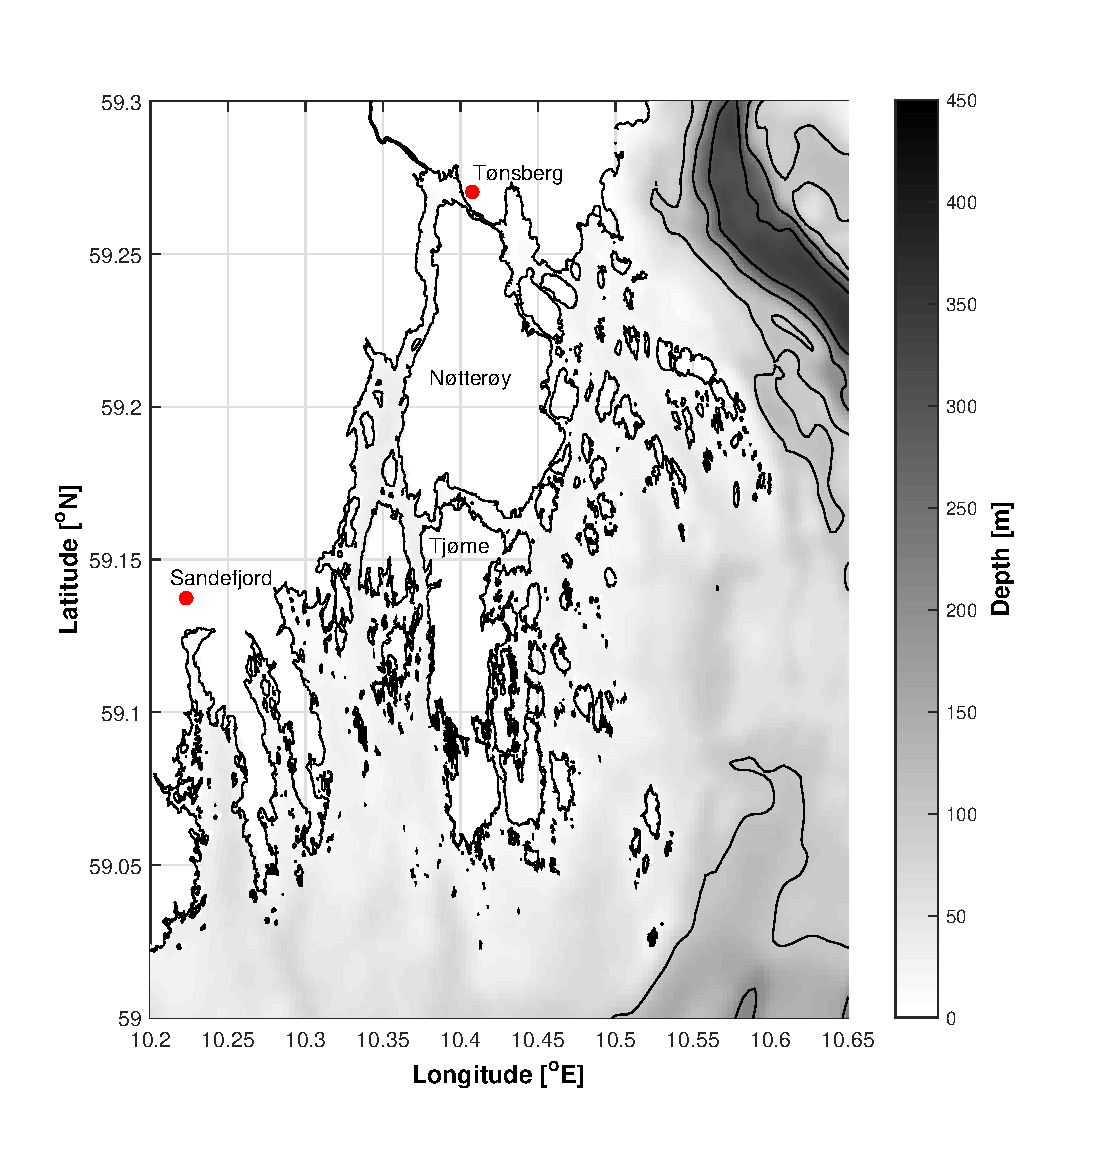
\includegraphics[height=8.5cm]{dyp_Tonsberg}}
   \rput[bl](7.5,0){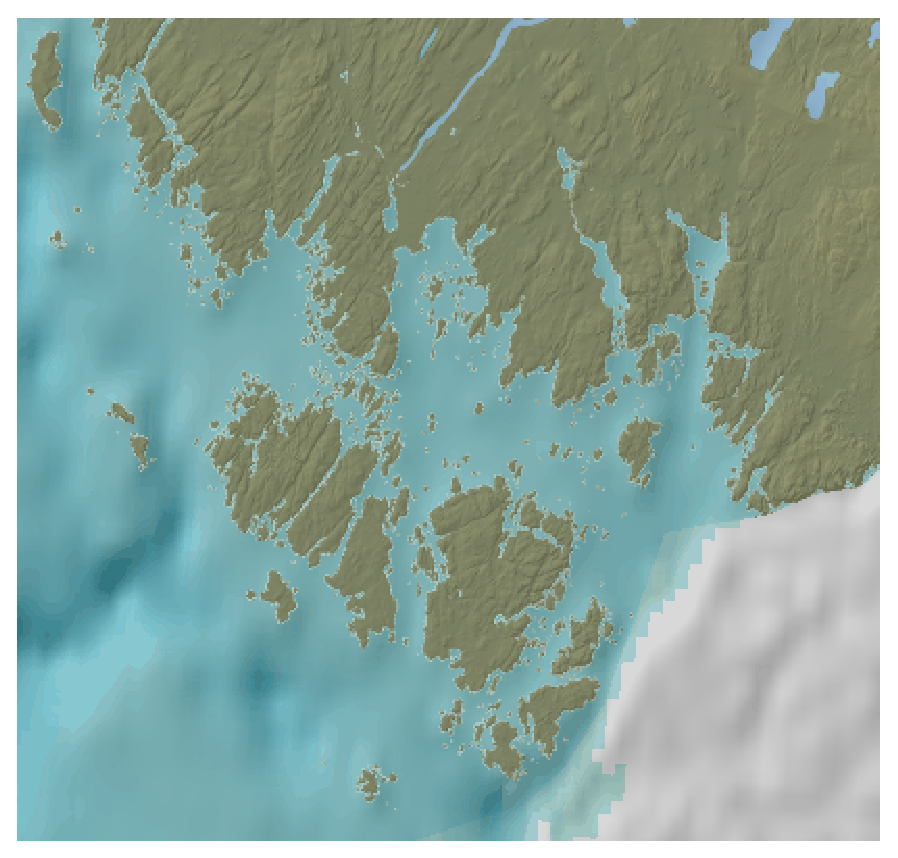
\includegraphics[height=8.5cm]{dyp_Hvaler}}
   \rput[bl](0,7){\large \textbf{a)}}
   \rput[bl](7.5,7){\large \textbf{b)}}
  \end{pspicture}
  \caption{\small a) The irregular coastline geometry and topography in the a) F{\ae}rder National Park and b) the Hvaler National Park. The grayscale in color bars indicates depth in meters. Note the many islands, narrow straits and channels present in these areas of the Oslofjord.}
  \label{fig:ferder_hvaler}
 \end{center}
\end{figure}

 

In addition to the {\DR} Sill area there are other areas in the fjord that features many smaller and larger islands. For instance to the west we find the T{\o}nsberg Archipelago including Bol{\ae}rne, Store and Lille F{\ae}rder (F{\ae}rder Lighthouse), and to the east we find Rauer and Hank{\o}, the Hvaler Archipelago and the smaller Islands S{\o}strene and Misingene (Figure \ref{fig:ferder_hvaler}). Further north on the west side of the fjord we find Bast{\o} south of Horten, and to the east Jel{\o}ya. Jel{\o}ya is separated from the mainland by a narrow channel about 50 m wide within which water sloshes back and forth with the tides \citep{hjelm:etal:2014}. The presence of these archipelagos with its small islands give rise to many narrow sounds, straits and channels impeding the water exchange. If the goal is to compute realistic pathways of any unwanted substances discharged to the fjord or trajectories of floating structures including man overboard (Search and Rescue Services), we need to resolve, to the best of our ability, these features. 

Finally it is worth mentioning the many rivers discharge freshwater to the fjord. For instance two of Norway's largest rivers, namely Glomma and Drammenselva\footnote{Here it is chosen to use Norwegian river names in which ``elv'' or ``vassdrag'', means ``river'' or ``water course''.}, are emptying their freshwater into the Oslofjord with a mean discharge of 729 and 317 m$^3$/s, respectively \citep{milli:etal:2011}. This freshwater has a decisive impact on the salinity and hence on the circulation in the fjord. Furthermore, in most fjords the river outlet is located at the fjord head leading to an estuarine circulation. In contrast the Glomma outlet is located in the outer part of the Oslofjord within the Hvaler Archipelago, while the Drammenselva outlet is located in the middle part of the fjord. As a result the estuarine circulation in the Oslofjord deviates considerably from a classical textbook example.        
%%%%%%%%%%%%%%%%%%%%%%%%%%% Figure 3 Godafoss %%%%%%%%%%%%%%%%%%%%%%%%%%%%%%%
\begin{figure}[t]
 \begin{center}
  \begin{pspicture}(0,0)(15,5.5)
% Include graphs
   \rput[bl](0.0, 0.0){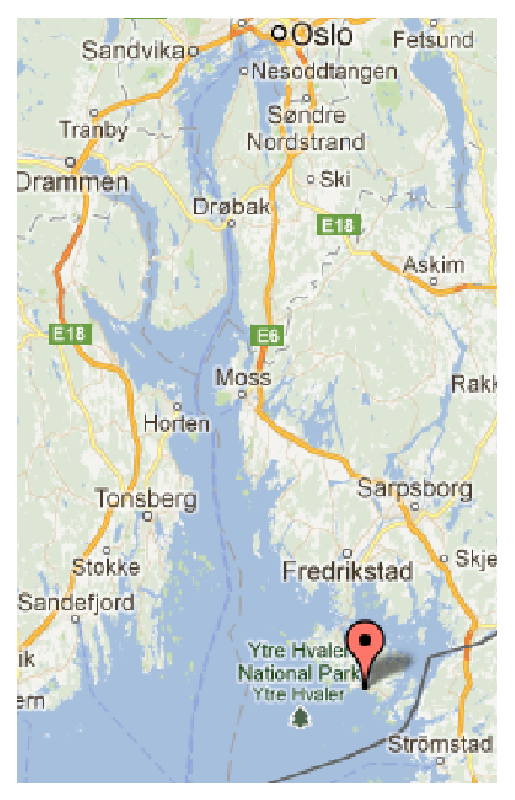
\includegraphics[height=5.5cm]{Fig03}}
   \rput[br](15.0,0.0){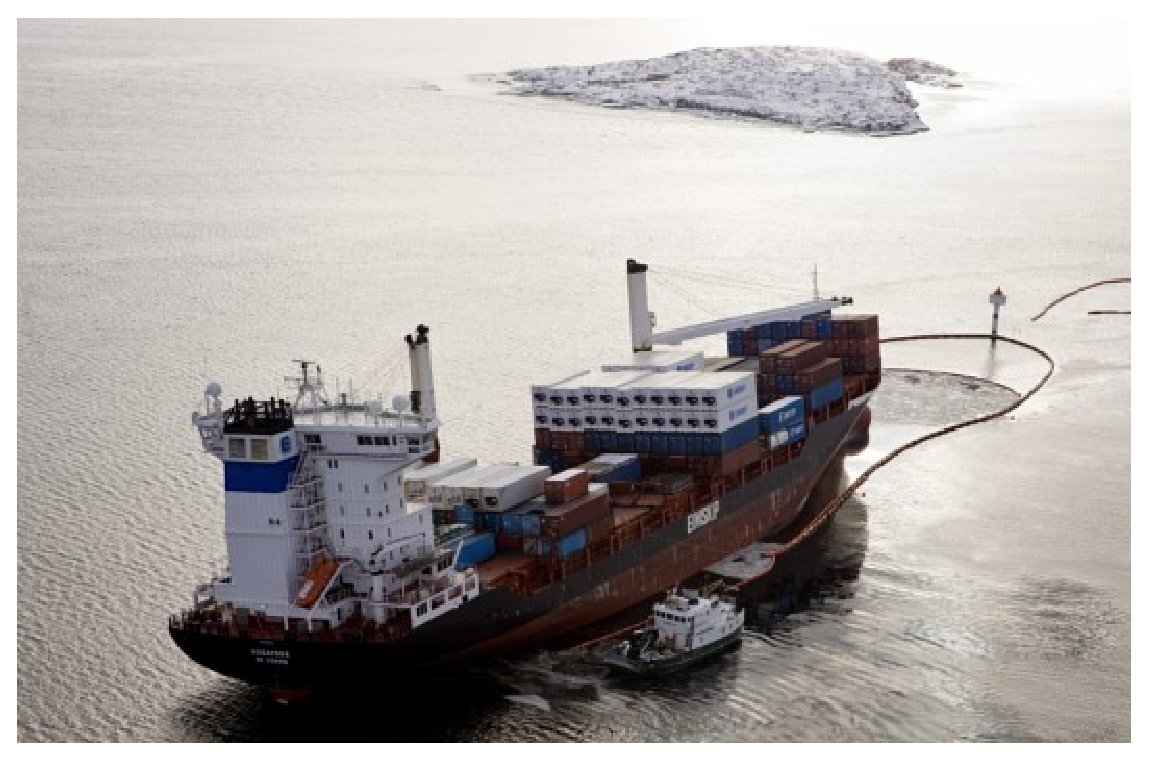
\includegraphics[height=5.5cm]{Fig03_2}}
  \end{pspicture}
  \caption{\small Map (left) showing the location where the ship ``Godafoss'' (right) grounded February 17, 2011. The location is in the sound L{\o}peren between two of the major islands in the Hvaler Archipelago where Norway's largest river flows through on its way to the Oslofjord.} 
  \label{fig:godafoss}
 \end{center}
\end{figure}



% % % % % % % % % % % % % % % % % % % % % % % % % % % % % % % % 
\subsection{Why a new model?}
\label{subsec:why}
The Oslofjord is somewhat special among the Norwegian fjords from a physical as well as a societal perspective. The population surrounding it, or more precisely people living less than one hours drive from the Oslofjord, comprises 40\% of the Norwegian population according to the official statistics\footnote{\texttt{http://www.ssb.no} as of July 1, 2012}. This is by far the most populated area in Norway, a population that is steadily growing. Moreover, no other fjord has anything close to as high density of leisure boats. In addition the Oslofjord features two of Norway's national underwater parks, the Hvaler National Park\footnote{\texttt{http://www.ytrehvaler.no/}} and the F{\ae}rder National Park\footnote{\texttt{http://prosjekt.fylkesmannen.no/faerdernasjonalpark/Om-Farder-nasjonalpark/}}. Thus, taking into account that the Oslofjord has the largest traffic density of commercial vessels of all the Norwegian fjords the risk of an accident resulting in a possible, unwanted contaminated effluent to the fjord is uncomfortably high. 
%%%%%%%%%%%%%%%%%%%%%%%%%%% Figure 3 Godafoss %%%%%%%%%%%%%%%%%%%%%%%%%%%%%%%
\begin{figure}[t]
 \begin{center}
  \begin{pspicture}(0,0)(15,10)
% Include graphs
   \rput[b](7.7, 0.0){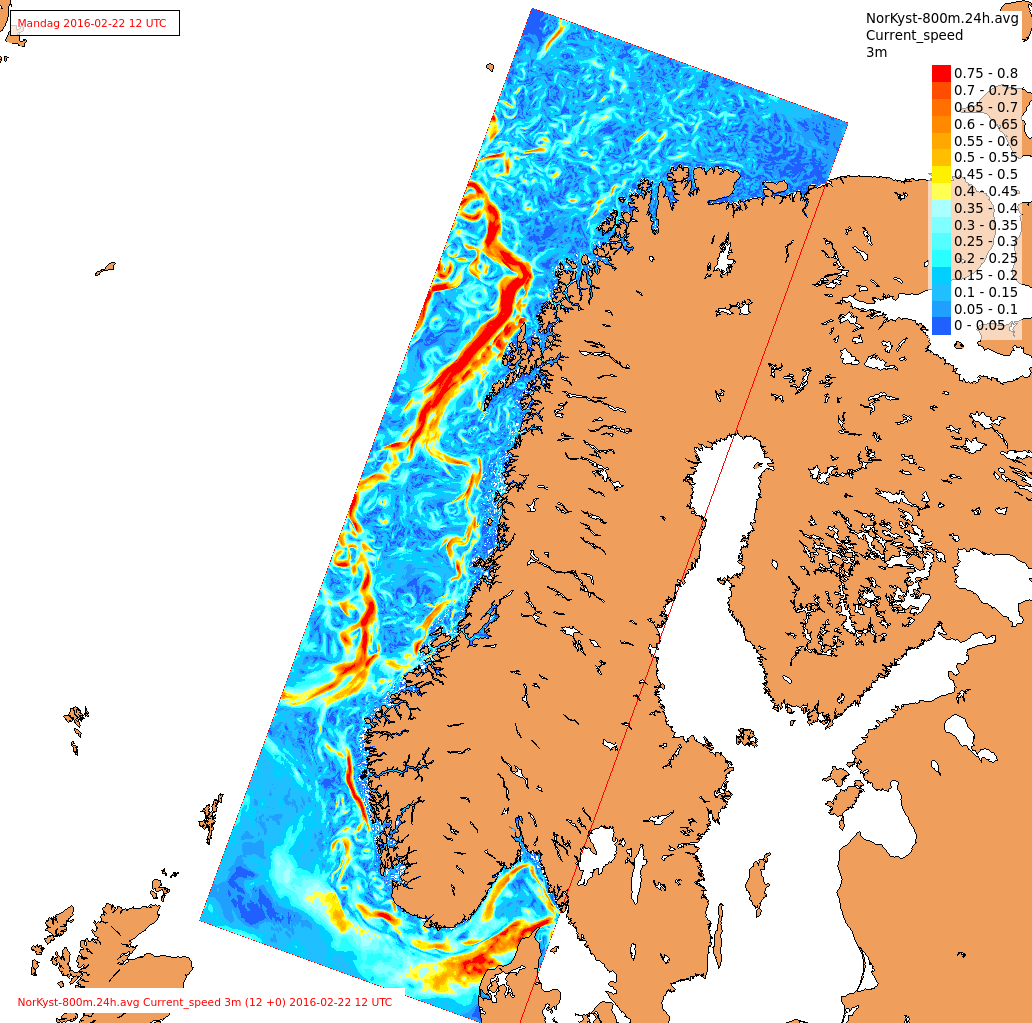
\includegraphics[height=10cm]{N800_2016-02-22_SPEED_3m_24h_avg}}
  \end{pspicture}
  \caption{\small The area covered by the NorKyst800 model. Shown is forecasted, 24 hour average speed at 3 m depth valid for February 22, 2016. Color bar gives speed in m/s with a a contour interval of 0.05 m/s.} 
  \label{fig:n800}
 \end{center}
\end{figure}

 

An example of such an unwanted event is the Godafoss accident. On February 17, 2011 the ship ``Godafoss'' grounded in a narrow sound in the Hvaler Archipelago (Figure \ref{fig:godafoss}), and a lot of its fuel oil leaked into the fjord. As part of the governmental emergency preparedness MET Norway's task is to forecast the dispersion, drift and spreading of the oil no later than half an hour after the accident\footnote{On behalf of the Norwegian Coastal Administration (Kystverket)}. As a matter of fact most of the accidents like Godafoss tend to happen close to the coast or within archipelagos\footnote{\texttt{https://en.wikipedia.org/wiki/List\_of\_oil\_spills}}. The safety of the people that utilize the fjord, and the protection of its environment, is therefore a challenge to governmental agencies, regional administrations and local management alike. 

Together with wind and waves ocean currents and temperature are key inputs to the model used to forecast oil drift. The present forecasting model providing the latter for the Oslofjord, and run operationally by MET Norway, is the NorKyst800 model \citep{albre:etal:2011}. As depicted by Figure \ref{fig:n800} it covers the entire Norwegian coast and not only the Oslofjord. In fact it was not developed to capture details within the Norwegian fjords, but rather to capture mesoscale phenomena such as jet currents, eddies and meanders along the the Norwegian coast outside of the fjords. It was set-up with a regular grid of 800x800 m, a grid of high  enough resolution to resolve the Rossby radius of deformation required to capture the mesoscale phenomena in Norway's near coastal waters. Nevertheless, due to its relatively high resolution of 800 m, it was still able to provide forecasts showing some skill even within the fjords.
%%%%%%%%%%%%%%%%%%%%%%%%%%% Figure 3 Godafoss %%%%%%%%%%%%%%%%%%%%%%%%%%%%%%%
\begin{figure}[t]
 \begin{center}
  \begin{pspicture}(0,0)(15,11)
% Include graphs
   \rput[br](7.4,5.5){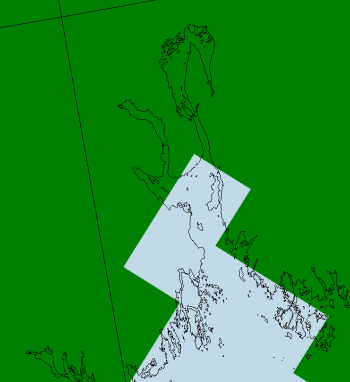
\includegraphics[height=5.2cm]{Oslofjord_A20_grid}}
   \rput[bl](7.5,5.5){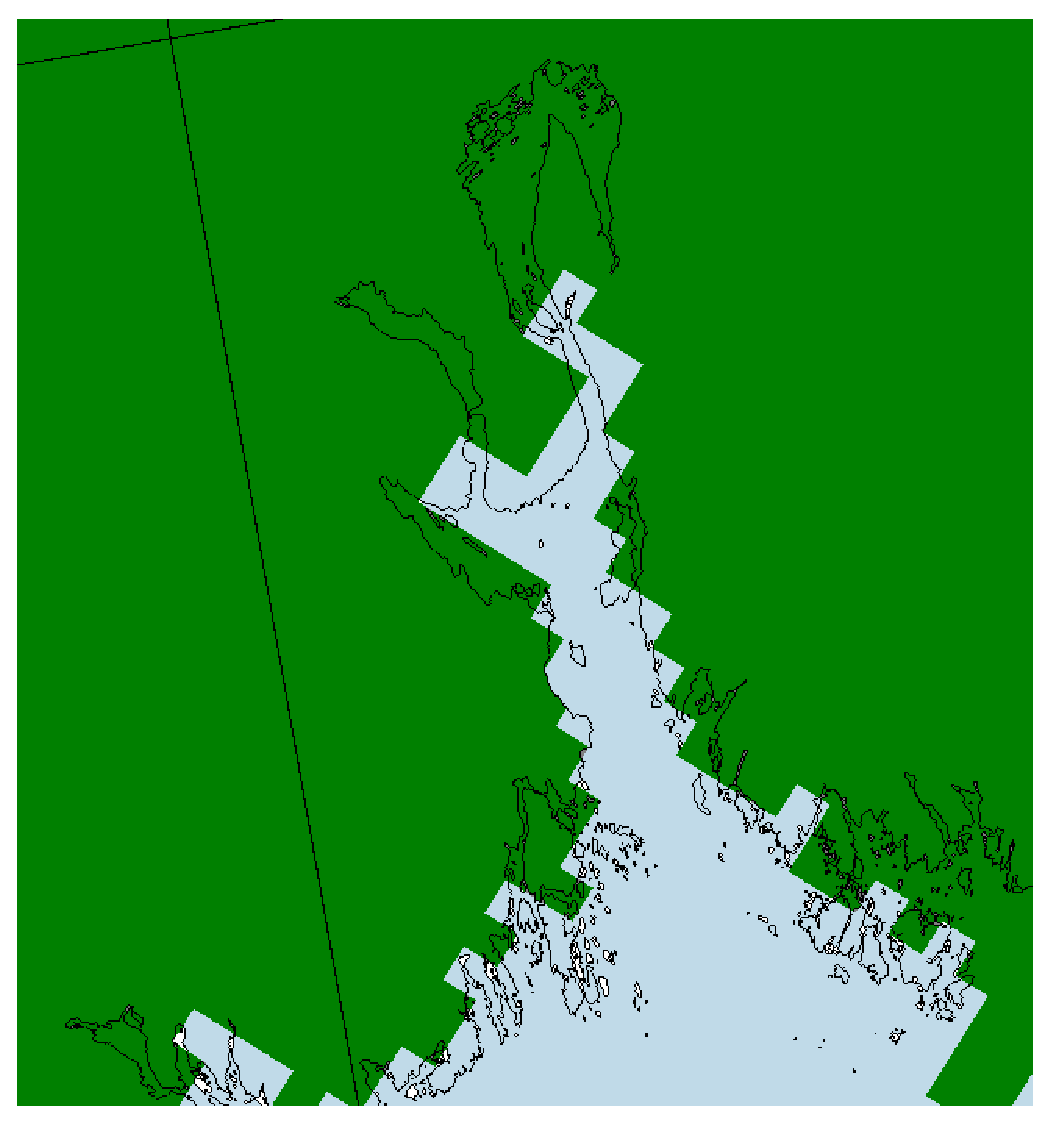
\includegraphics[height=5.2cm]{Oslofjord_N4_grid}}
   \rput[br](7.4,0.0){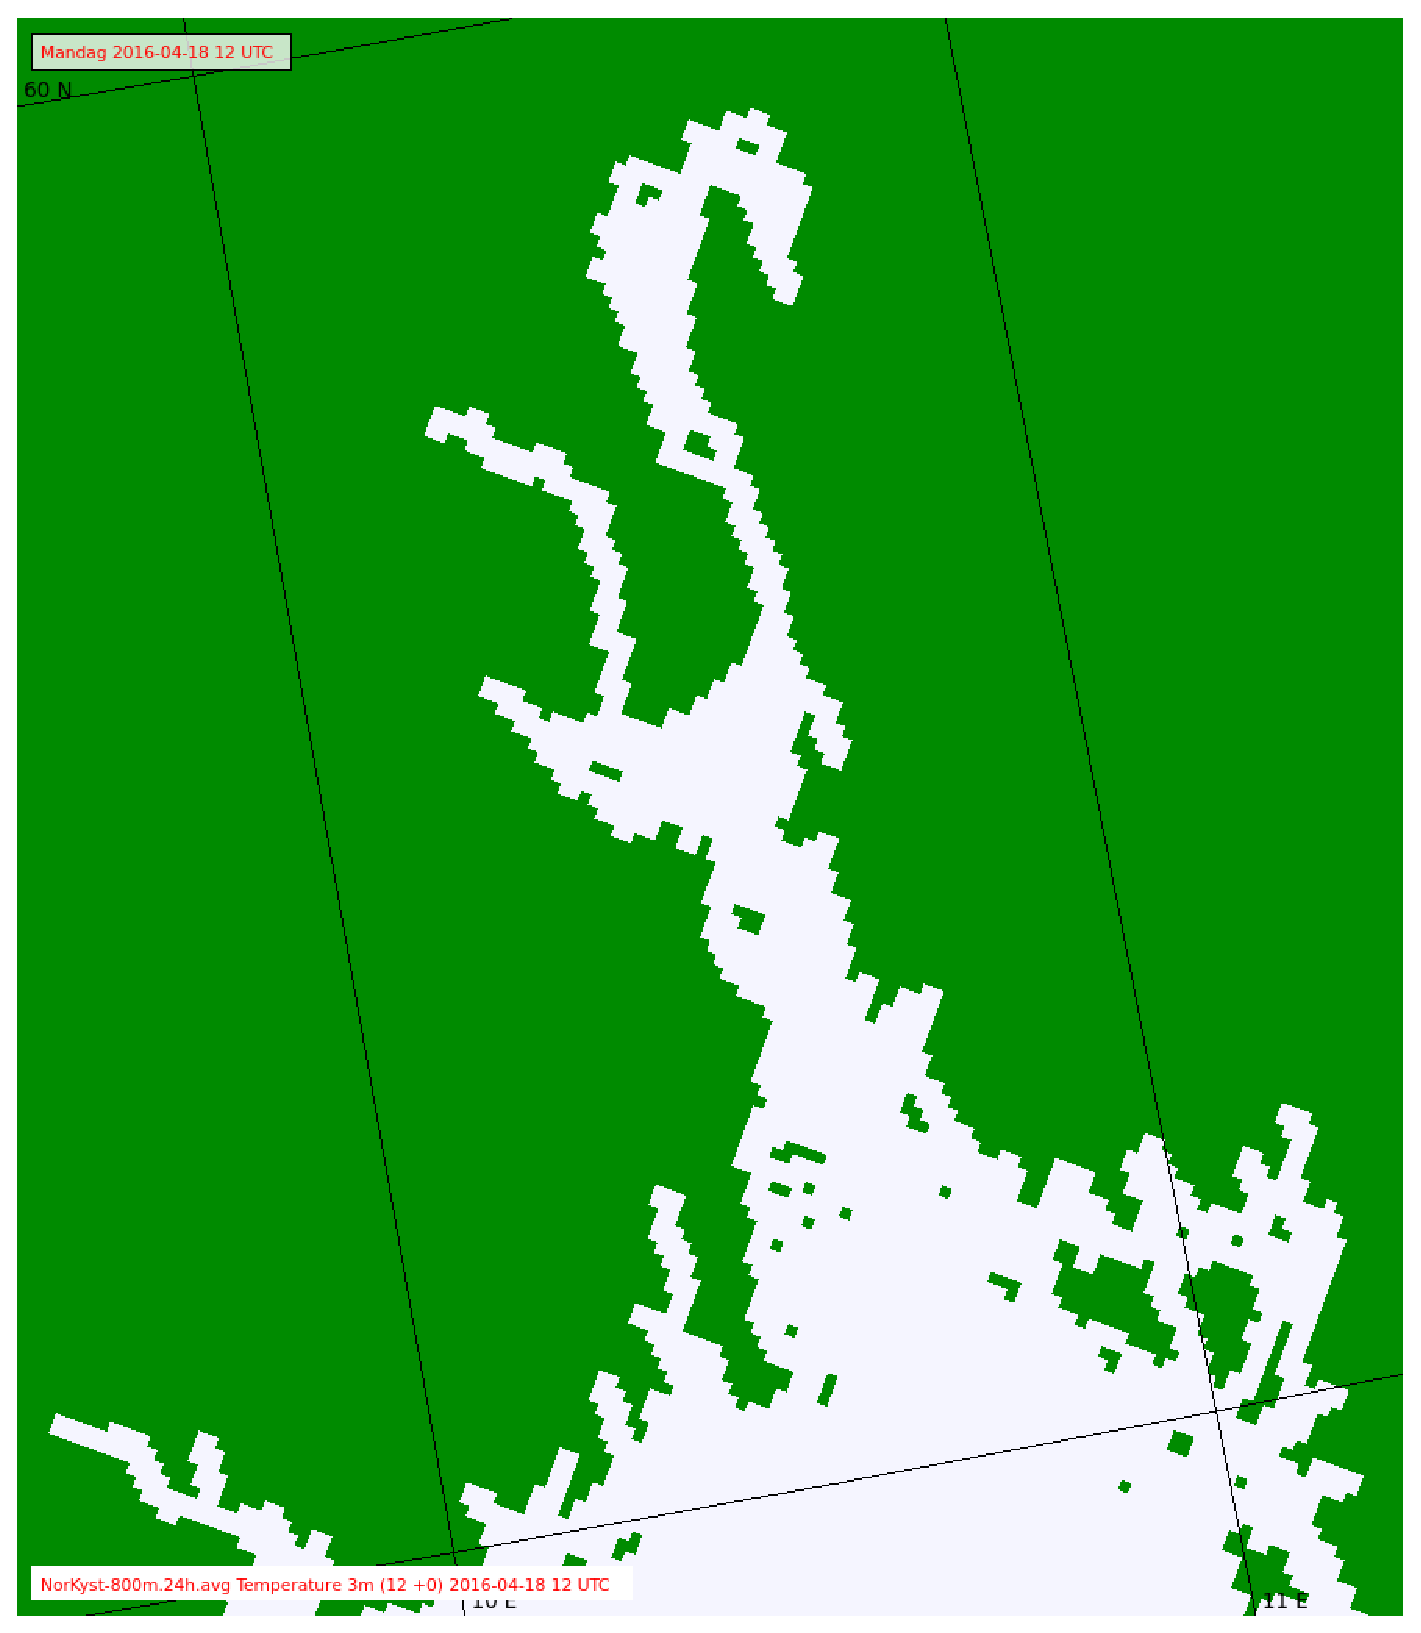
\includegraphics[height=5.2cm]{Oslofjord_N800_grid}}
   \rput[bl](7.5,0.0){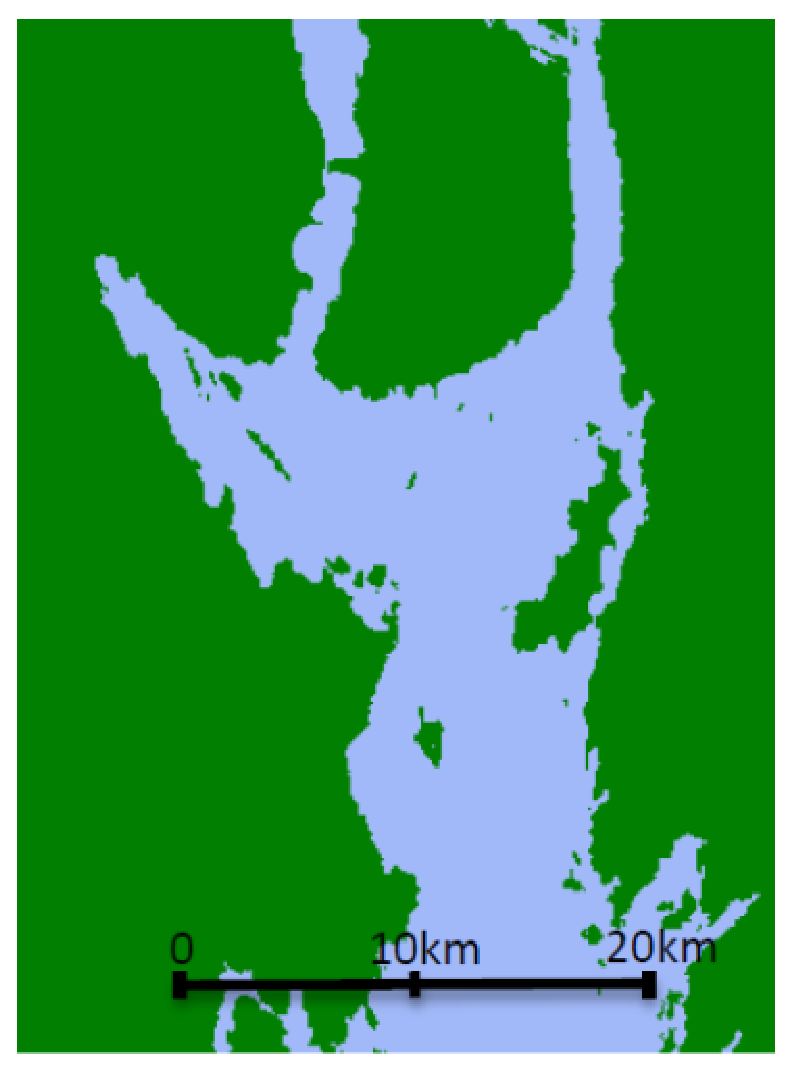
\includegraphics[height=5.2cm]{Midfjord_100m_grid}}
  \end{pspicture}
  \caption{\small Illustrated is the impact of grid resolution on how the Oslofjord is portrayed. Upper two (from left to right) show how the fjord is represented by respectively a 20 km and 4 km grid model, while the two tbottom panels show the same for respectively an 800 m and 100 m grid model zoomed in on Breidangen.} 
  \label{fig:resolution}
 \end{center}
\end{figure}



Despite NorKyst800's relatively high resolution it is still not fine enough to resolve the highly irregular geometry and topography of most Norwegian fjords, and the Oslofjord is no exception. These irregularities consist of small islands, narrow sounds, straits and channels and many smaller scale deep basins and shallow sills as alluded to in Section \ref{subsec:oslofjord} (Figure \ref{fig:map_oslofj}). To properly forecast oil drift, or dispersion of any unwanted substances or contaminants accidentally discharged to the fjord, it is therefore of utmost importance that the underlying fjord model has a realistic representation of the majority of these irregularities. 

The aim of the project FjordOs is therefore to develop an Oslofjord model to resolve most of these features without requiring excessive computer power. We emphasize that such a model, if made operational, will benefit all governmental emergency preparedness models, including those operated by MET Norway. In addition to oil drift these are (i) Search And Rescue or SAR models, which involves forecasting of pathways of floating objects, e.g., man overboard, rafts, small crafts and ships, (ii) transport and spreading of dissolved substances such as nutrients and toxic substances (e.g., nuclear waste), and (iii) growth and drift of toxic algae. Finally we emphasize that resolving the fine scale, submesoscale motion due to the fjord's irregular geometry and topography is required to avoid floating objects, dissolved substances and oil from stranding artificially.  

A vizualization of the impact of resolution on how well the model portrays these irregularities is depicted by Figures \ref{fig:resolution}. As is evident it is only the 100 m grid that represents the Oslofjord as we know it from geographical charts and maps. An example is the small islands in Breidangen (Tofteholmen and M{\o}len simply not present in the 800 m grid model. Likewise the shape and area covered by Bast{\o}y is improved in the 100 m grid, and so is the ridge that cuts into the the Drammensfjord at Svelvik. The same is true regarding topography. An example is displayed by Figure \ref{fig:hvaler2} that compares the topography represented by the new Oslofjord model (FjordOs CL) and Norkyst800. 

To conclude today's forecasting model available for the Oslofjord (NorKyst800) has an insufficient resolution, and a new model of the Oslofjord with a resolution of 100 m or less for most parts of the fjord is needed. The development of a such a model would also greatly benefit all governmental emergency preparedness models including those operated by MET Norway.   
%%%%%%%%%%%%%%%%%%% Figure 2 Bathymetry and currents in the Drøbak area %%%%%%%%%%%%%%%
\begin{figure}[t]
 \begin{center}
  \begin{pspicture}(0,0)(15,8.5)
% Include graphs
   \rput[tl](-0.1,9.5){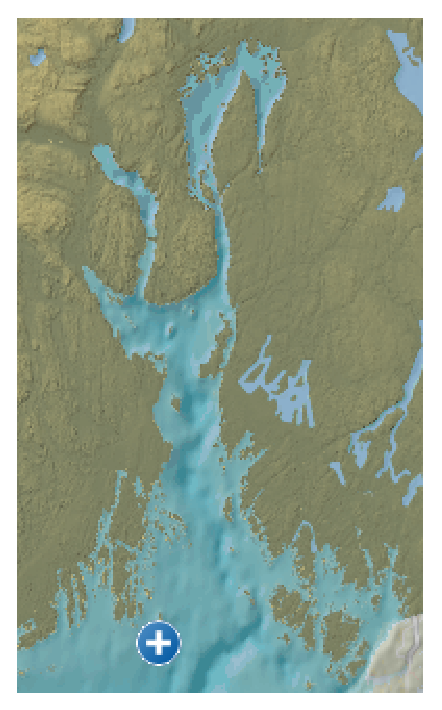
\includegraphics[height=8.5cm]{dyp}}
   \rput[tr](  15,9.5){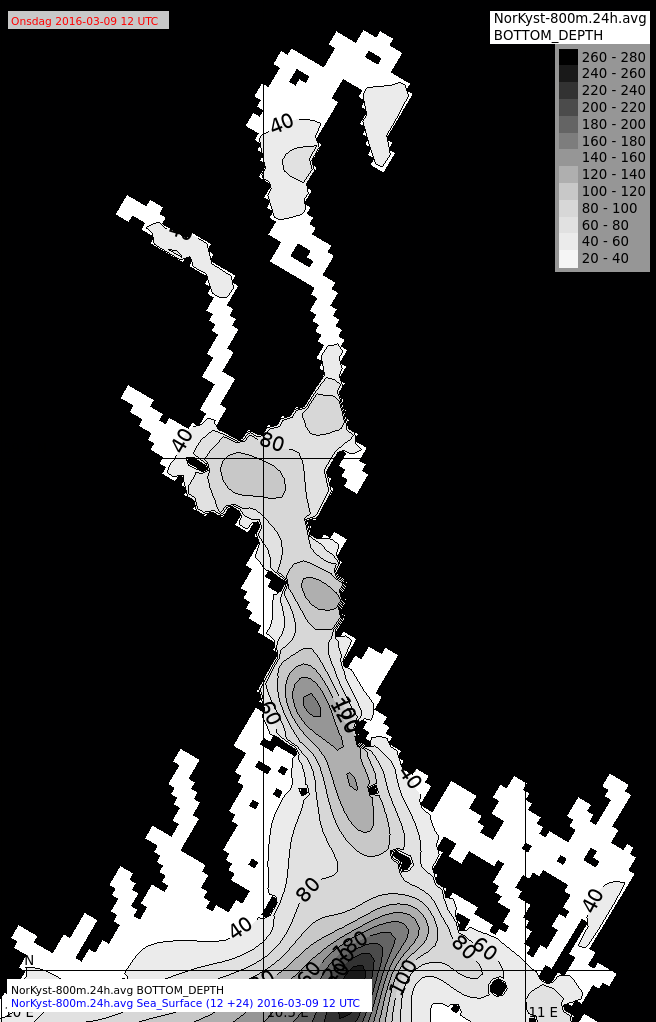
\includegraphics[height=8.0cm]{NorKyst800_topo_oslofjord}}
  \end{pspicture}
  \caption{\small The irregular coastline geometry and topography in the Oslofjord as portrayed in the FjordOs CL model (left) and the NorKyst800 model (right). The color bar (grayscale) indicate depth in meters.}
  \label{fig:hvaler2}
 \end{center}
\end{figure}



% % % % % % % % % % % % % % % % % % % % % % % % % % % % % % % % 
\subsection{Organization of the report}
Notwithstanding that the purpose of this report is to document the technical details regarding the development of the new Oslofjord model FjordOs CL, we have included above some of the characteristics of the Oslofjord (Section \ref{subsec:why}), and provided some of the motivation why a new Oslofjord model is needed (Section \ref{subsec:oslofjord}). Section \ref{sec:model} provides some details on how the curvilinear grid of the FjordOs CL model is constructed. Section \ref{sec:setup} provides some model specifics while Section \ref{sec:forcing} gives details on the model's bathymetry and external forcing such as tides, ocean input through open lateral boundaries, river input as well as atmospheric input. Section \ref{sec:resul} provides some results from an almost two year long hindcast and some test forecasts. Finally we offer a summary and some concluding remarks in Section \ref{sec:summa}. 
